% ------------------------------------------------------------------------------
% TYPO3 Version 10.3 - What's New (French Version)
%
% @license	Creative Commons BY-NC-SA 3.0
% @link		https://typo3.org/help/documentation/whats-new/
% @language	French
% ------------------------------------------------------------------------------

\section{Interface Utilisateur Backend}
\begin{frame}[fragile]
	\frametitle{Interface Utilisateur Backend}

	\begin{center}\huge{Chapitre 1~:}\end{center}
	\begin{center}\huge{\color{typo3darkgrey}\textbf{Interface Utilisateur Backend}}\end{center}

\end{frame}

% ------------------------------------------------------------------------------
% Feature | 90333 | Dashboard

\begin{frame}[fragile]
	\frametitle{Interface Utilisateur Backend}
	\framesubtitle{Tableau de bord (1)}

	Un tableau de bord montrant des informations système importantes à l'utilisateur
	authentifié est introduit.

	\begin{figure}
		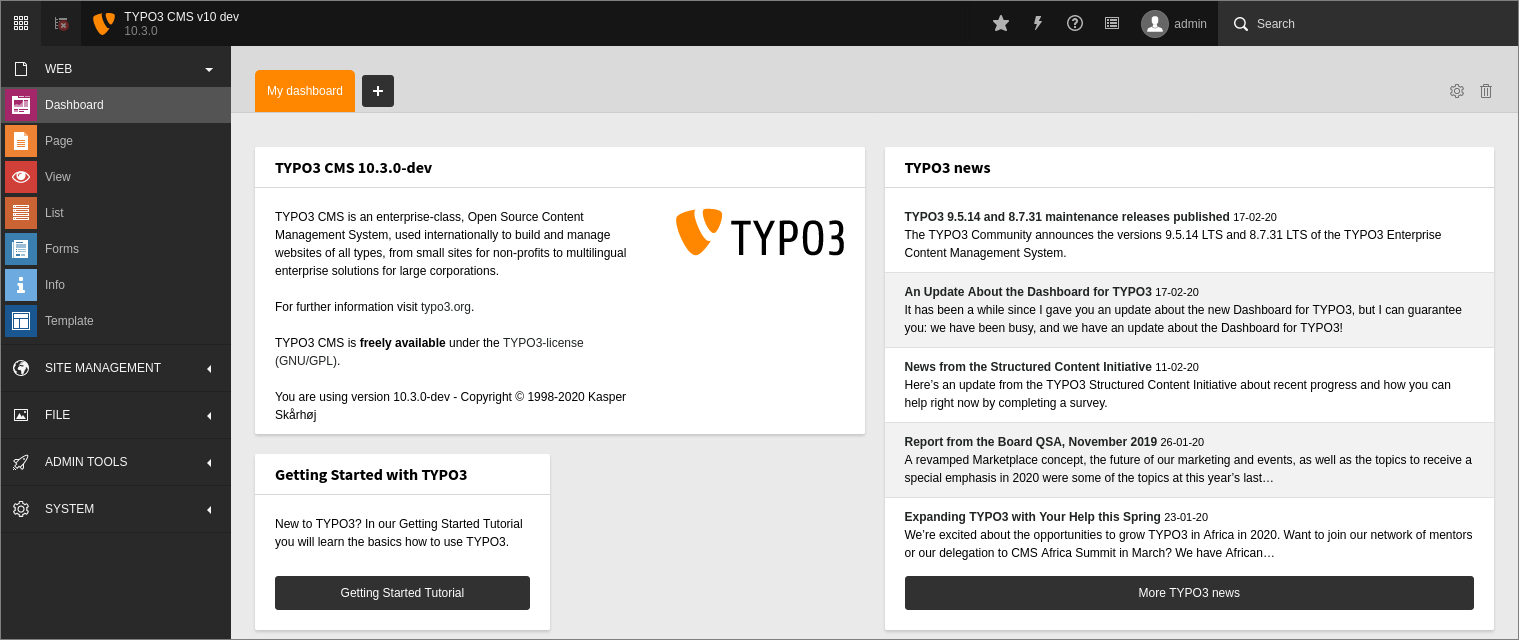
\includegraphics[width=1\linewidth]{BackendUserInterface/90333a-Dashboard.png}
	\end{figure}

\end{frame}

% ------------------------------------------------------------------------------
% Feature | 90333 | Dashboard

\begin{frame}[fragile]
	\frametitle{Interface Utilisateur Backend}
	\framesubtitle{Tableau de bord (2)}

	Les utilisateurs peuvent créer leur tableau de bord et y ajouter des
	widgets, en retirer et les réarranger.
	Les développeurs peuvent créer des widgets dans leurs extensions.

	\begin{figure}
		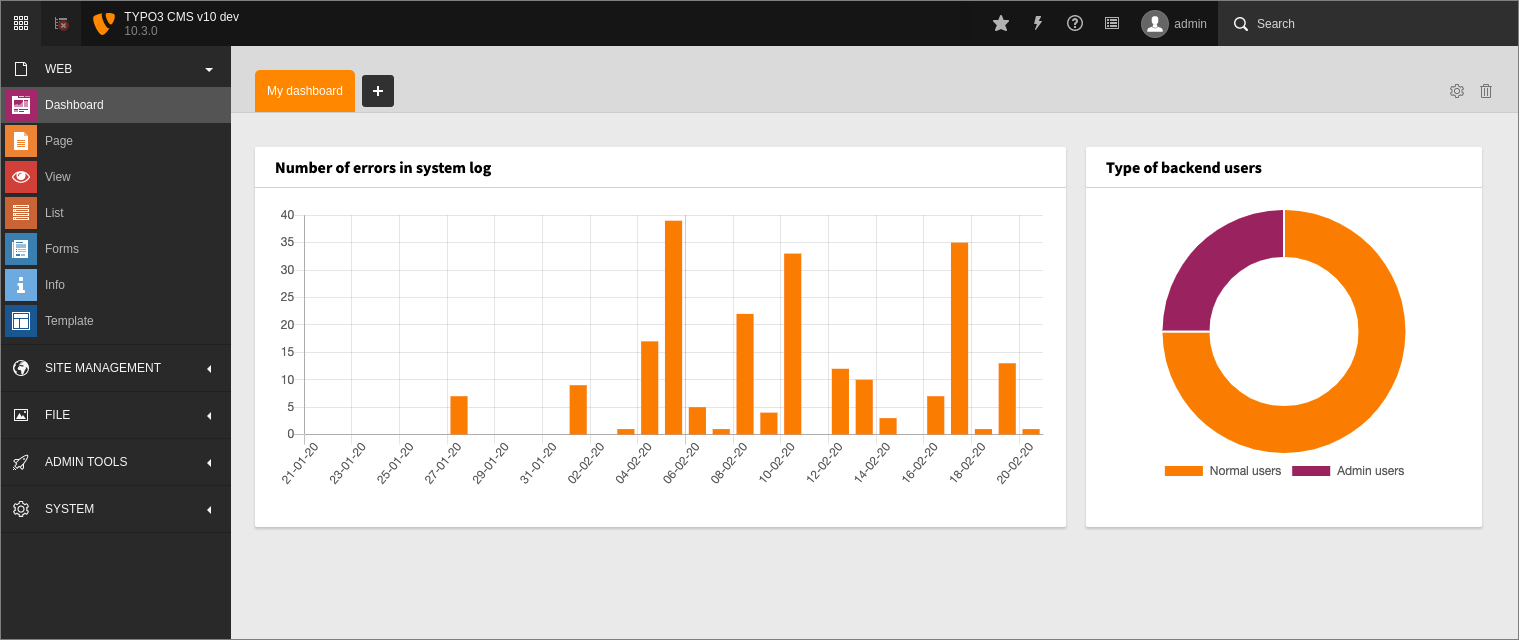
\includegraphics[width=1\linewidth]{BackendUserInterface/90333b-Dashboard.png}
	\end{figure}

\end{frame}

% ------------------------------------------------------------------------------
% Feature | 89513 | Provide password recovery for backend users
%
%\begin{frame}[fragile]
%	\frametitle{Interface Utilisateur Backend}
%	\framesubtitle{Récupération du mot de passe}
%
%	Les utilisateurs backend peuvent réinitialiser leurs mots de passe
%   en cas d'oublie.
%
%	\begin{figure}
%		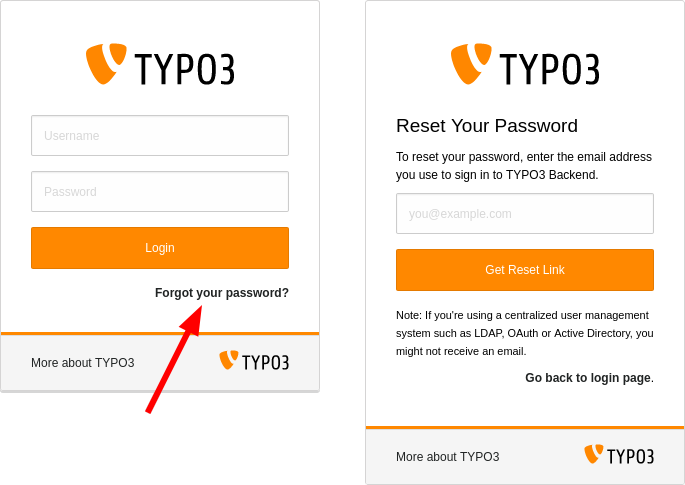
\includegraphics[width=0.6\linewidth]{BackendUserInterface/89513-ProvidePasswordRecoveryForBackendUsers.png}
%	\end{figure}
%
%\end{frame}
%
% ------------------------------------------------------------------------------
